\renewcommand{\documentname}{System design}

\chapter{System design}


Until now we have seen a theoretical view of the algorithms, with some pseudocode, and an abstracted technical view of the system with the analysis discussed in the previous session. This chapter presents to the reader, with the help of different diagrams, a more technical side to the prototype in which the actual code of the utility will be based. The software architecture, the detailed class diagram and the format of the files used by the system follow.


\section{System architecture}

The architecture of the system is laid out in two diagrams, the component diagram, which models the relationship between the subsystems and their interfaces; and the package diagram, which shows the logical layout of the code.

The component diagram is depicted below.


\begin{figure}[H]
    \caption{Components diagram}
  \centering
  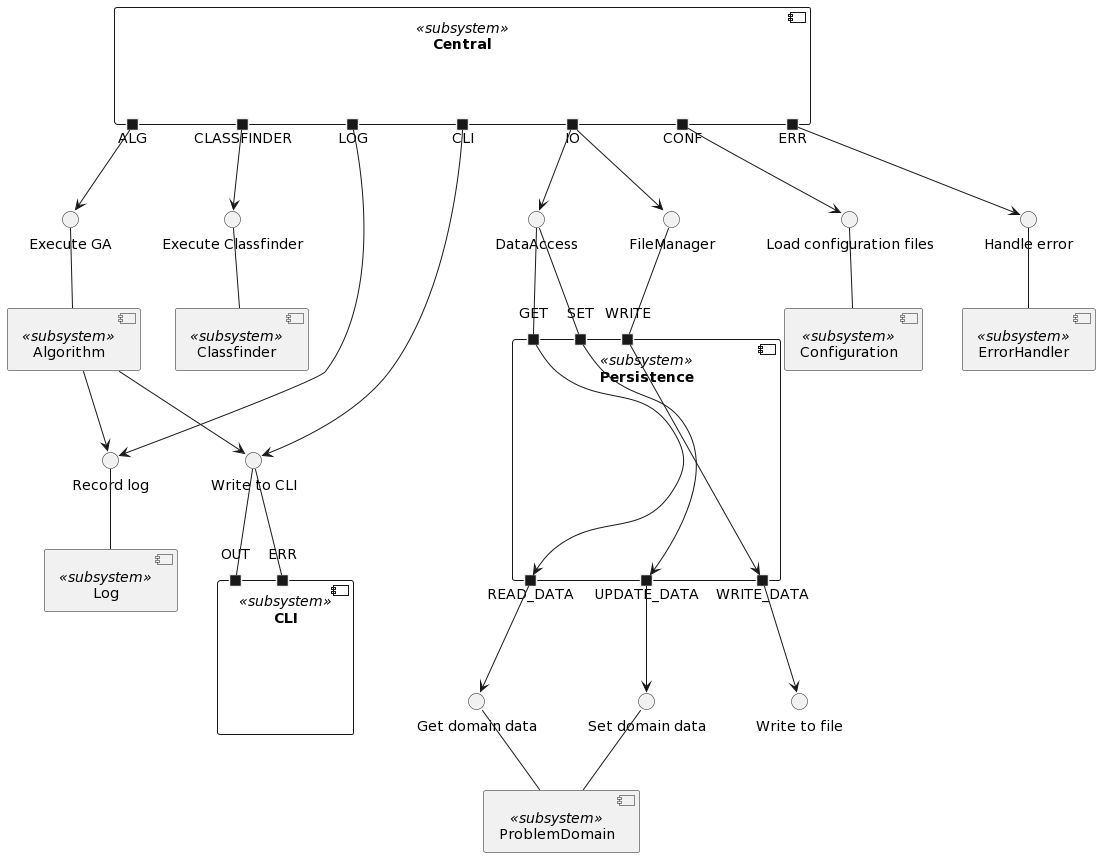
\includegraphics[scale=0.4]{components_diagram_uml.png}
\end{figure}

It can be seen that the central subsystem is responsible for connecting the major subsystems with each other, especially those belonging to the different code layers. Only the central subsystem and the algorithm subsystem have direct access to the log and the CLI.

The relationship between the persistence layer and the problem domain subsystem is due to the fact that it is the former that creates the data for the latter, and once the central subsystem receives this data, it is responsible for providing said data to the different components that require it.

Thus, the package diagram follows.

\begin{figure}[H]
    \caption{Packages diagram}
  \centering
  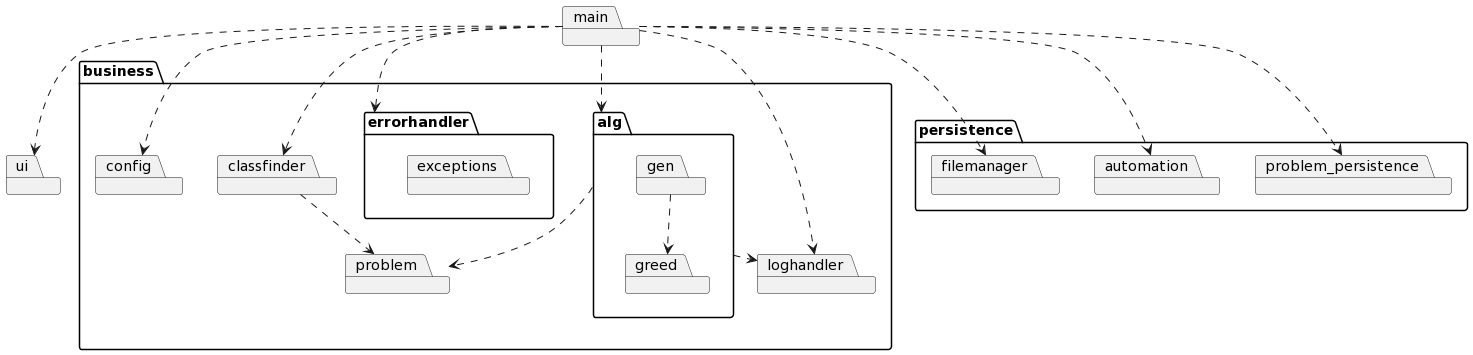
\includegraphics[scale=0.3]{packages_diagram_uml.png}
\end{figure}

What is noteworthy of this diagram is the appearance of new elements that the initial class diagram did not have. For example, the error handler contains both its logic and the definition of the prototype's own exceptions. The log handler contains a reference to the internal Java log logic, and acts as a wrapper that facilitates communication with other modules. Finally, the persistence layer has three main packages: the file manager, in charge of writing and reading files; the automation functionality of the files from the School to our files; and finally the DataAccess to the files of the domain.




\section{Class design}

This section presents the different class diagrams that make up the whole system, without showing trivial details and without repeating elements with similar layouts, in order to enhance readability.


\begin{figure}[H]
    \caption{Class diagram: Alg package}
  \centering
  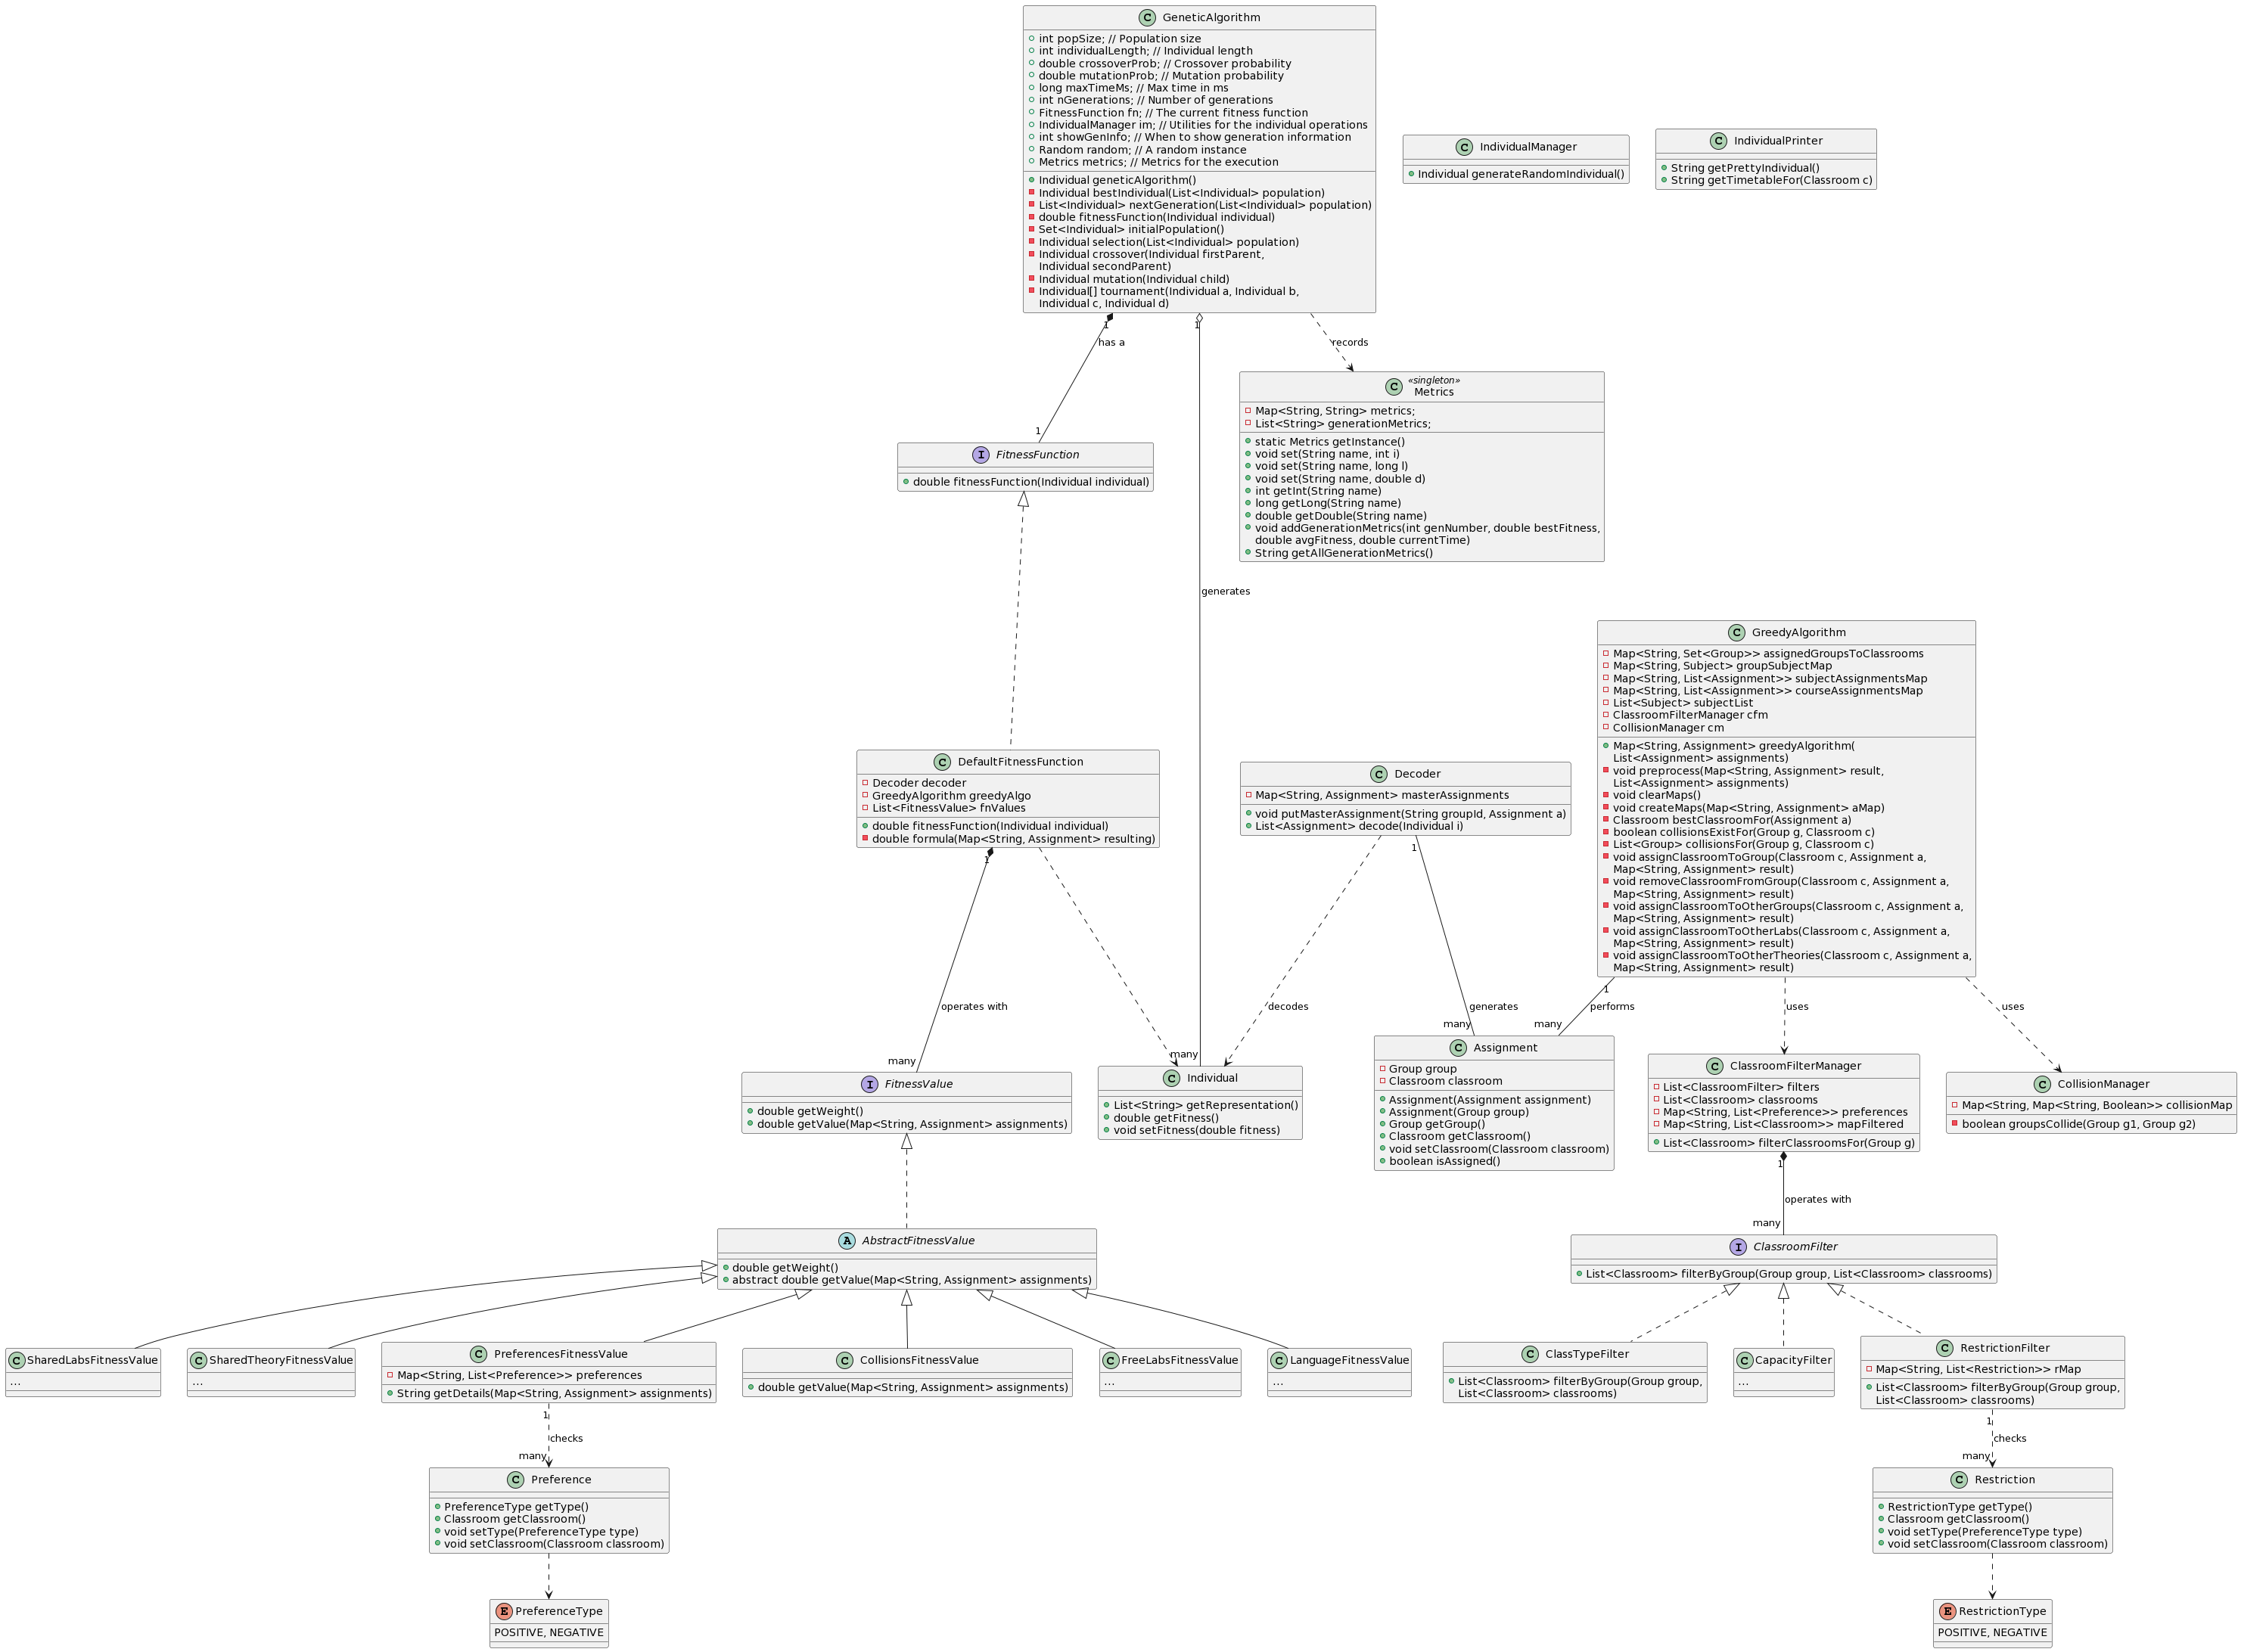
\includegraphics[scale=0.15]{final_alg_class_diagram_uml.png}
\end{figure}

\begin{figure}[H]
    \caption{Class diagram: Alg package (Greedy algorithm)}
  \centering
  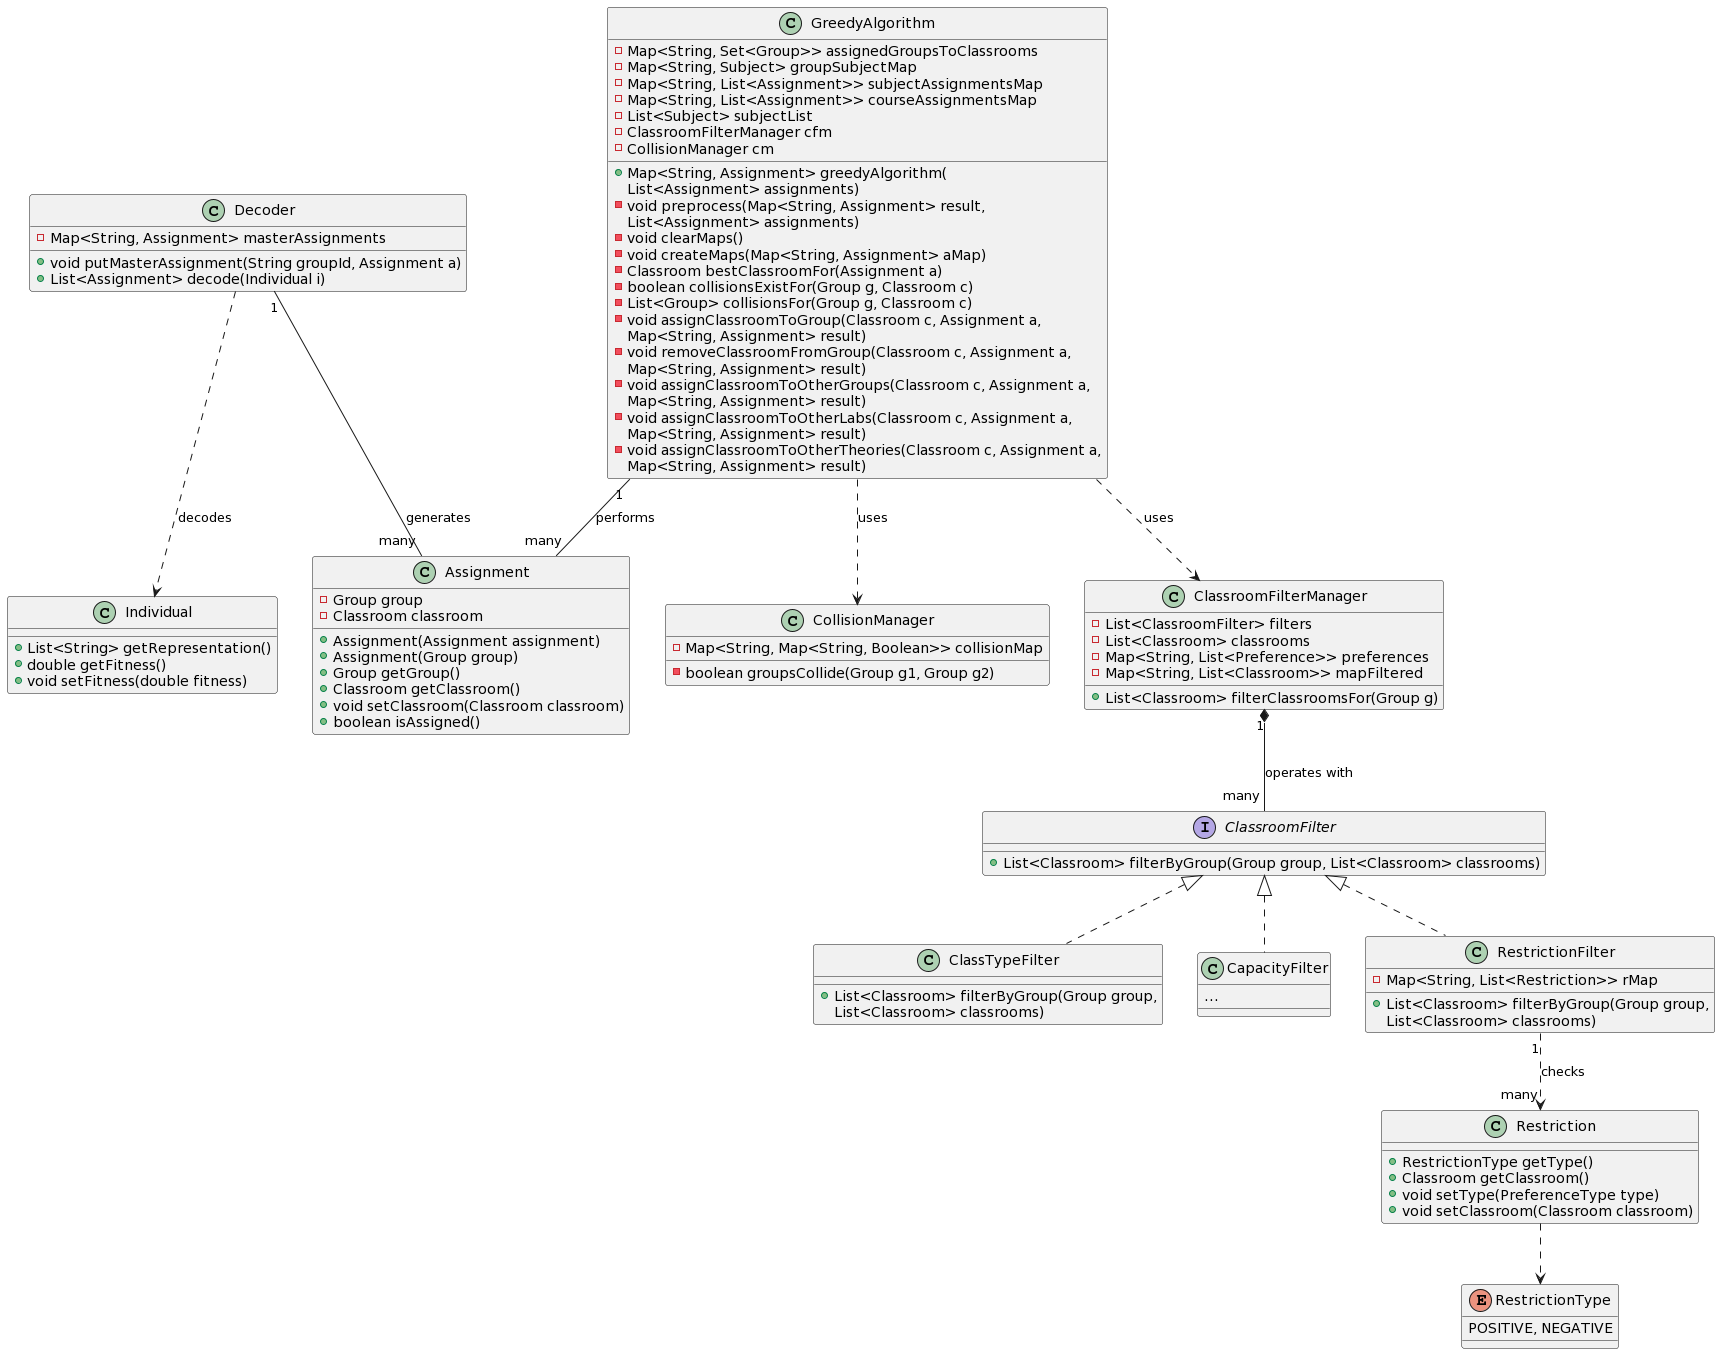
\includegraphics[scale=0.28]{final_alg_greedy_class_diagram_uml.png}
\end{figure}

\begin{figure}[H]
    \caption{Class diagram: Alg package (Genetic algorithm)}
  \centering
  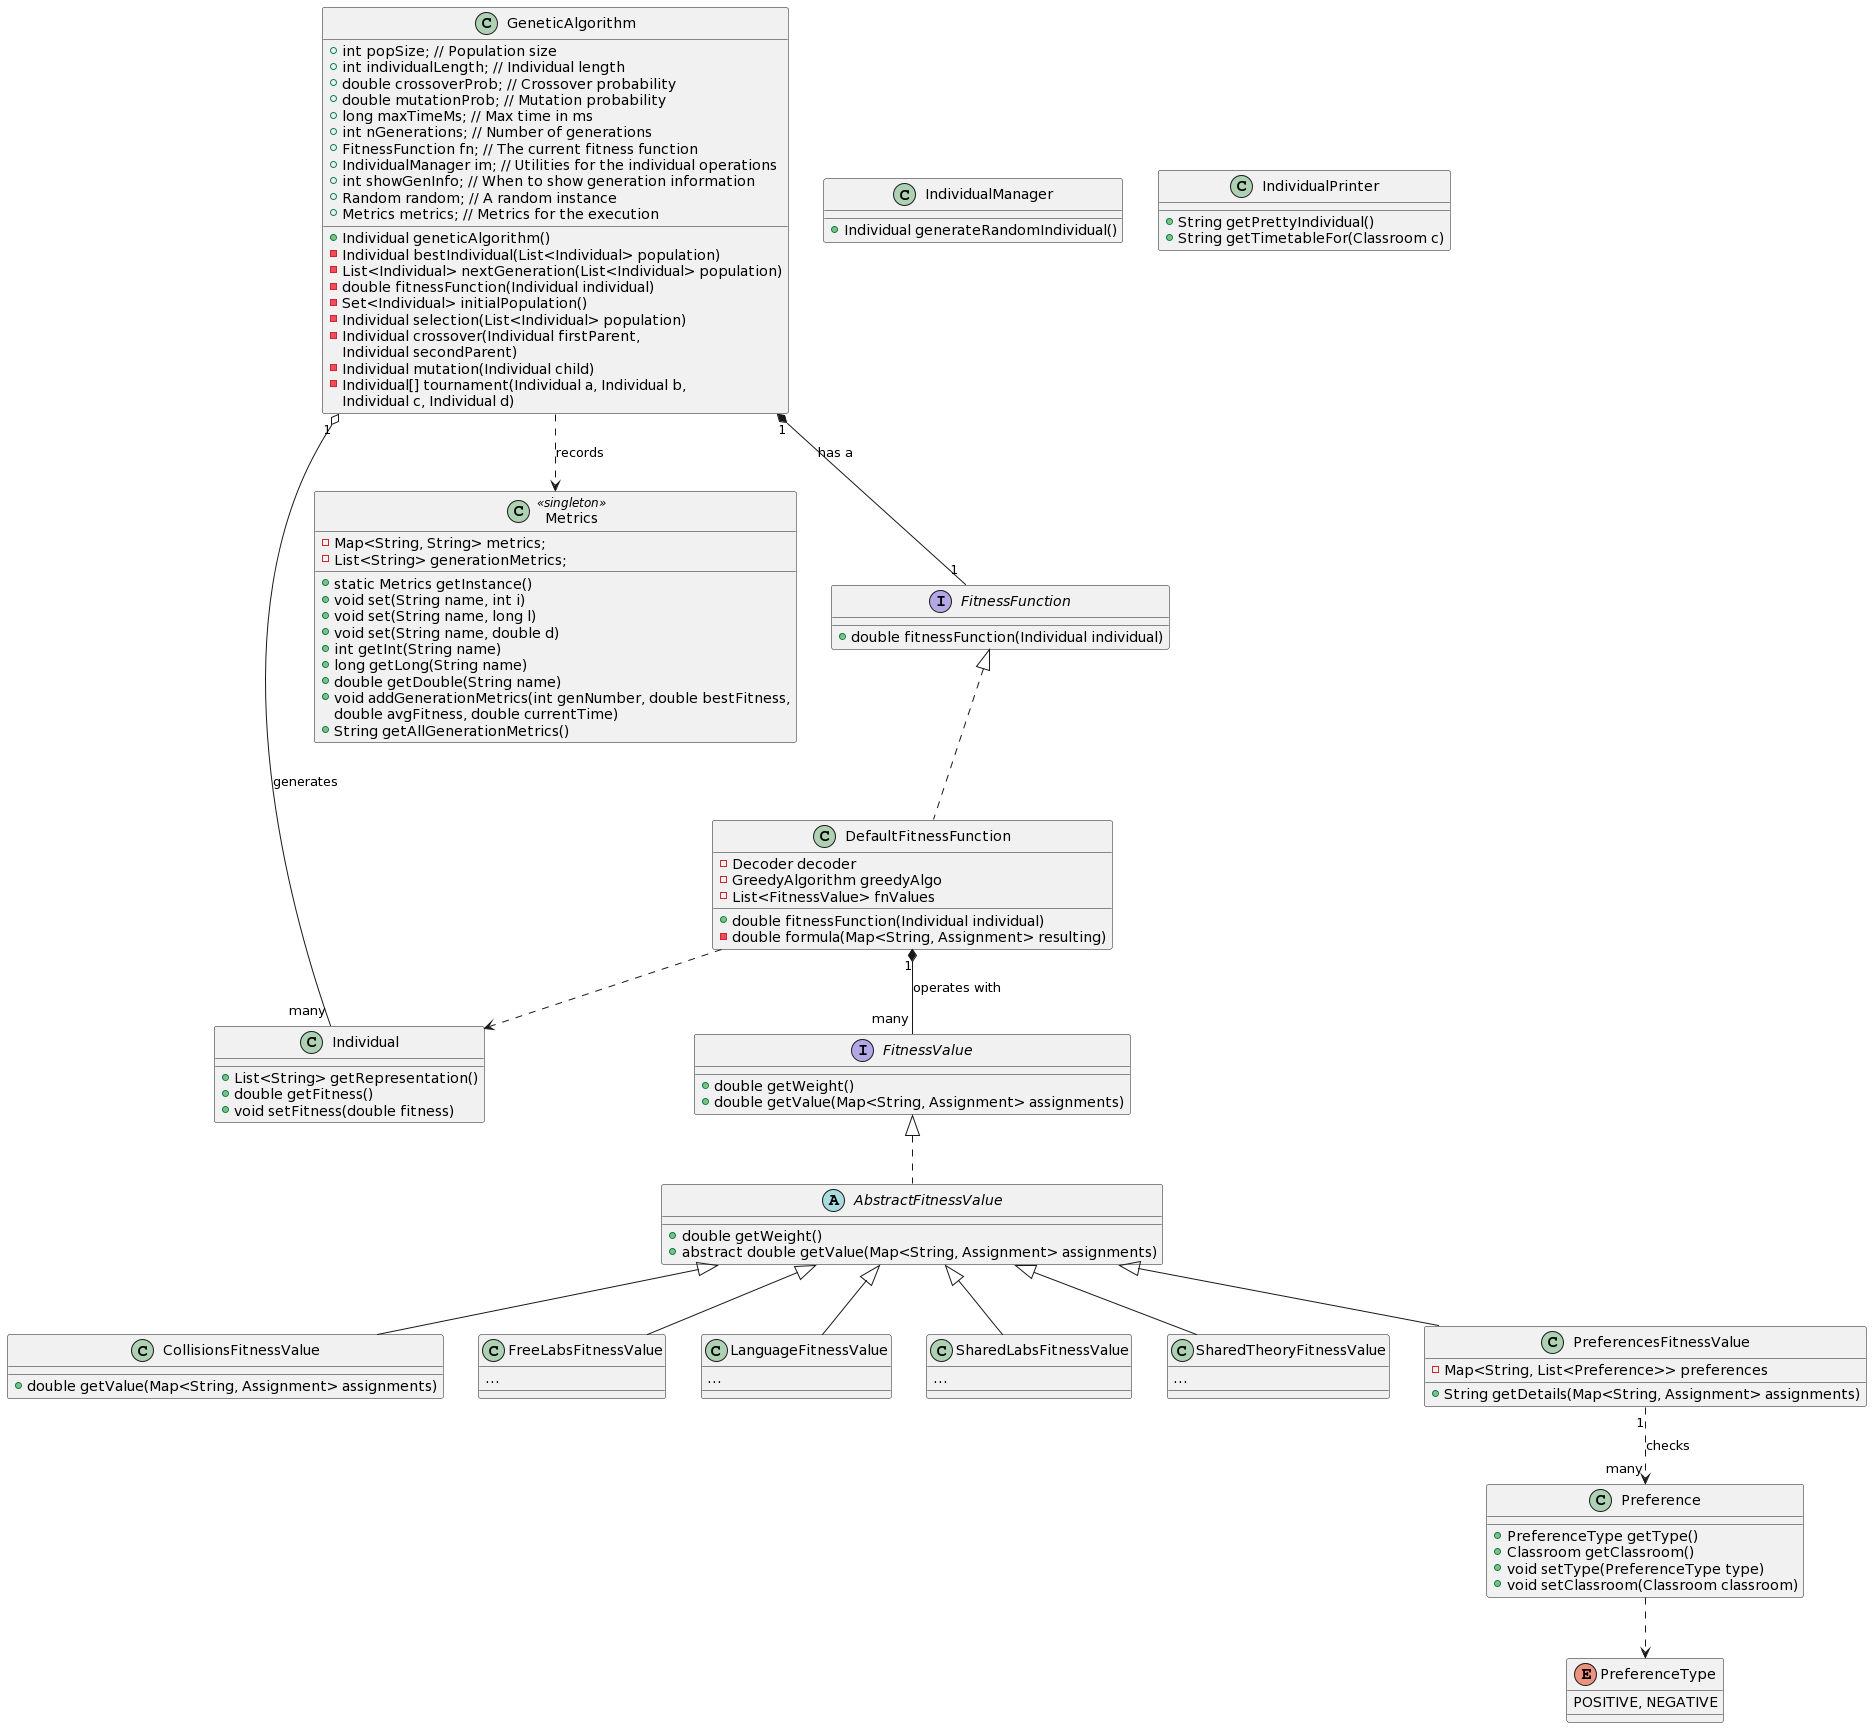
\includegraphics[scale=0.27]{final_alg_genetic_class_diagram_uml.png}
\end{figure}

\begin{figure}[H]
    \caption{Class diagram: Problem domain}
  \centering
  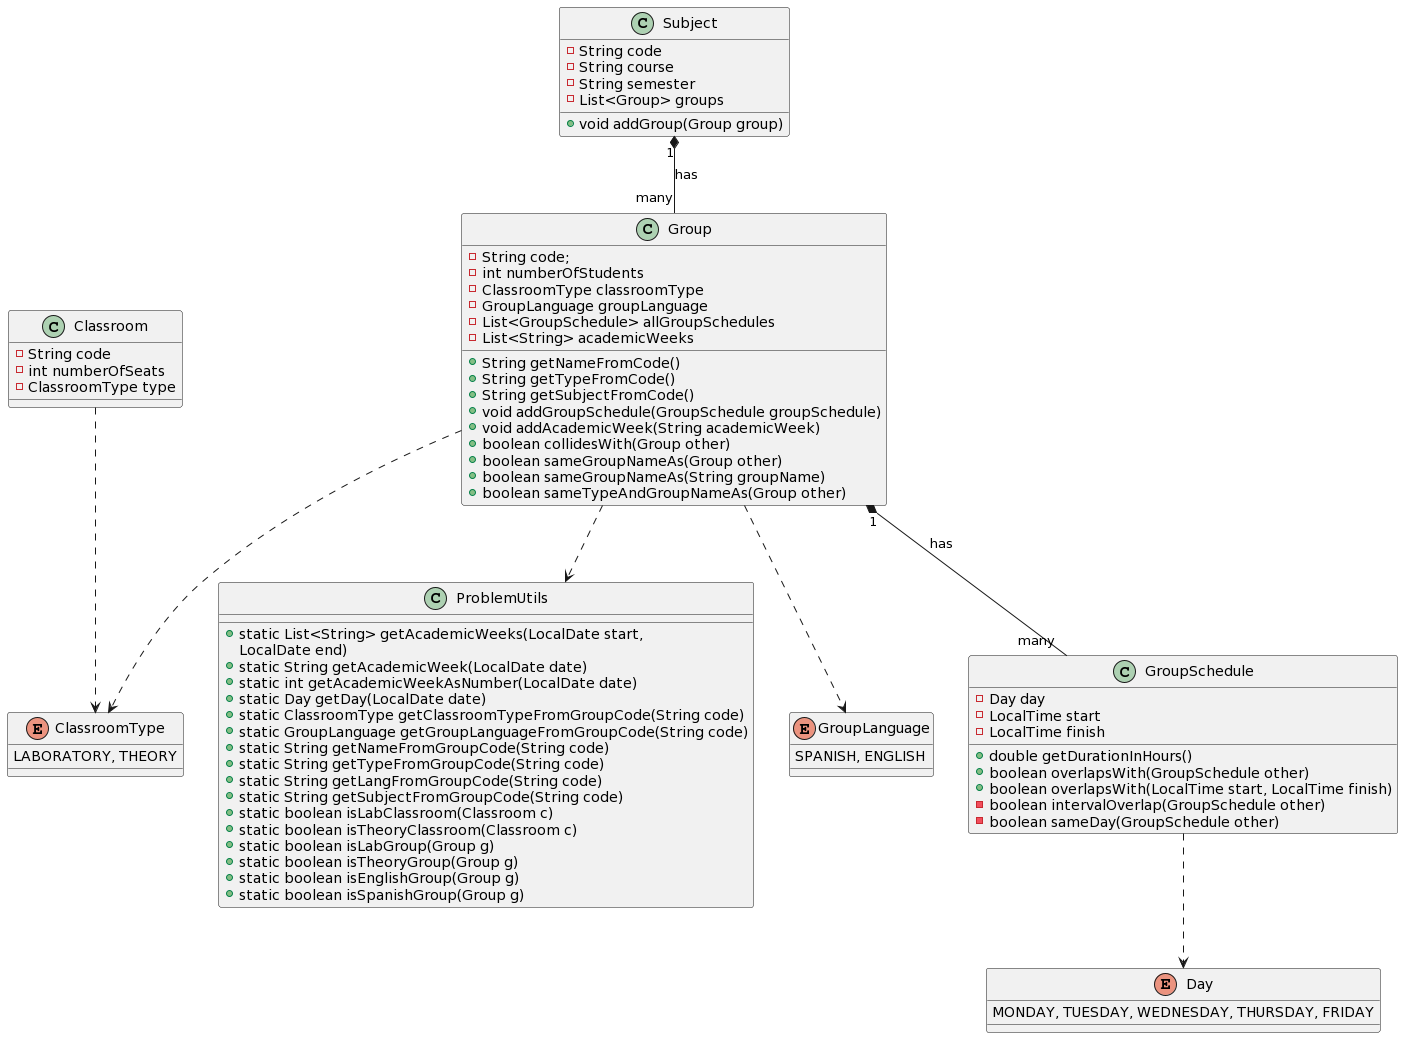
\includegraphics[scale=0.35]{final_problem_class_diagram_uml.png}
\end{figure}

\begin{figure}[H]
    \caption{Class diagram: Other business classes}
  \centering
  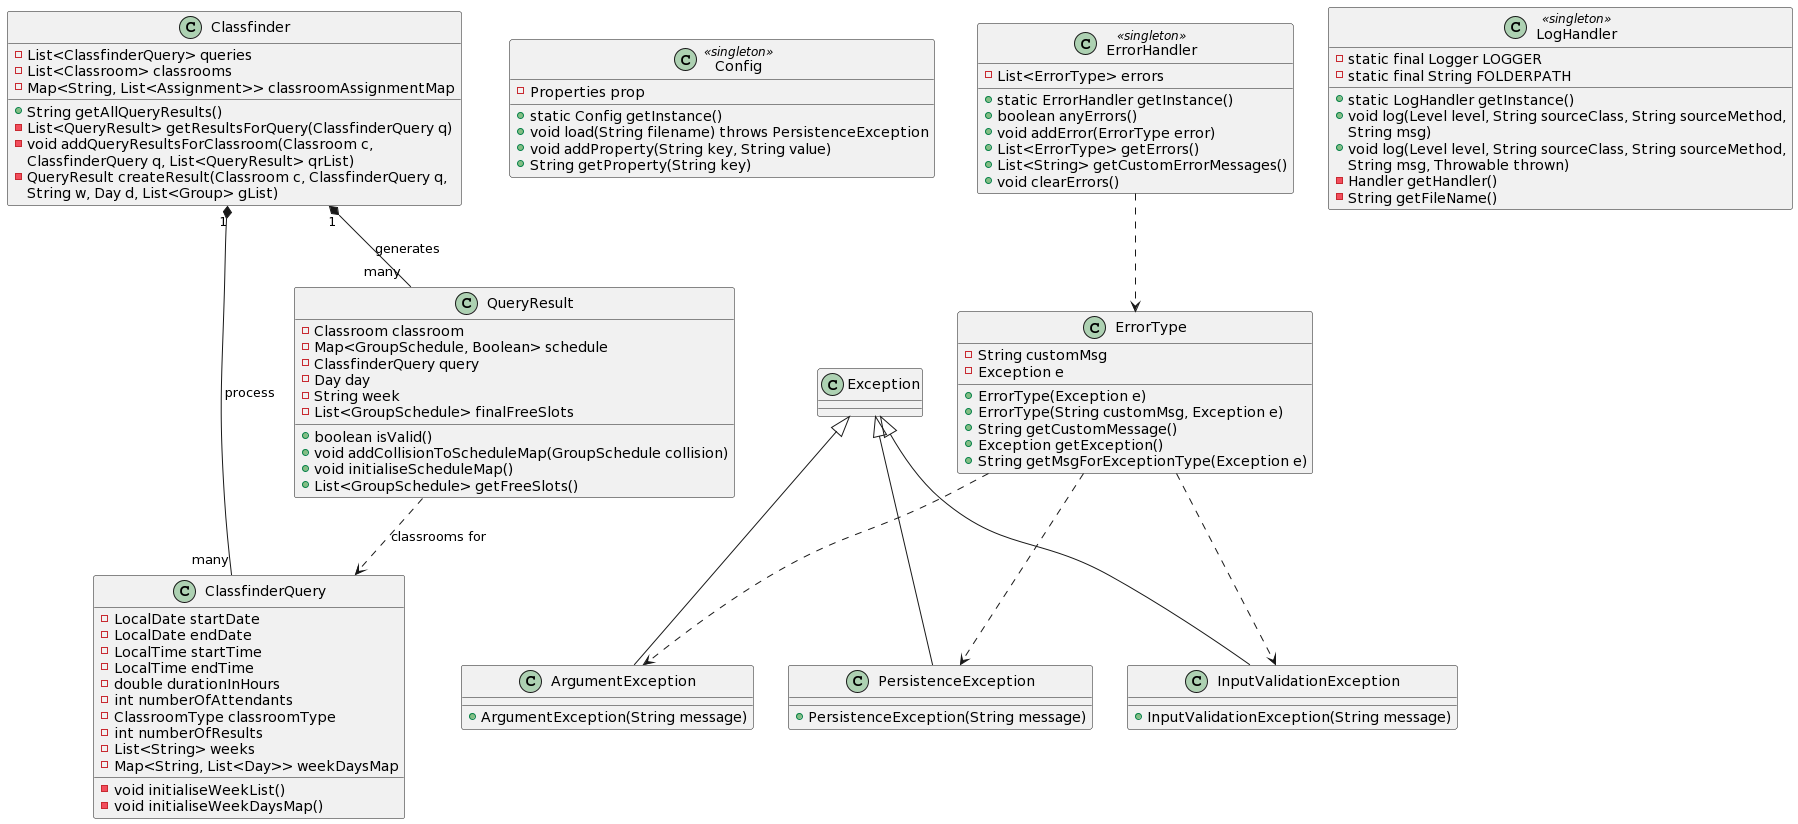
\includegraphics[scale=0.28]{final_business_other_class_diagram_uml.png}
\end{figure}

\begin{figure}[H]
    \caption{Class diagram: Persistence}
  \centering
  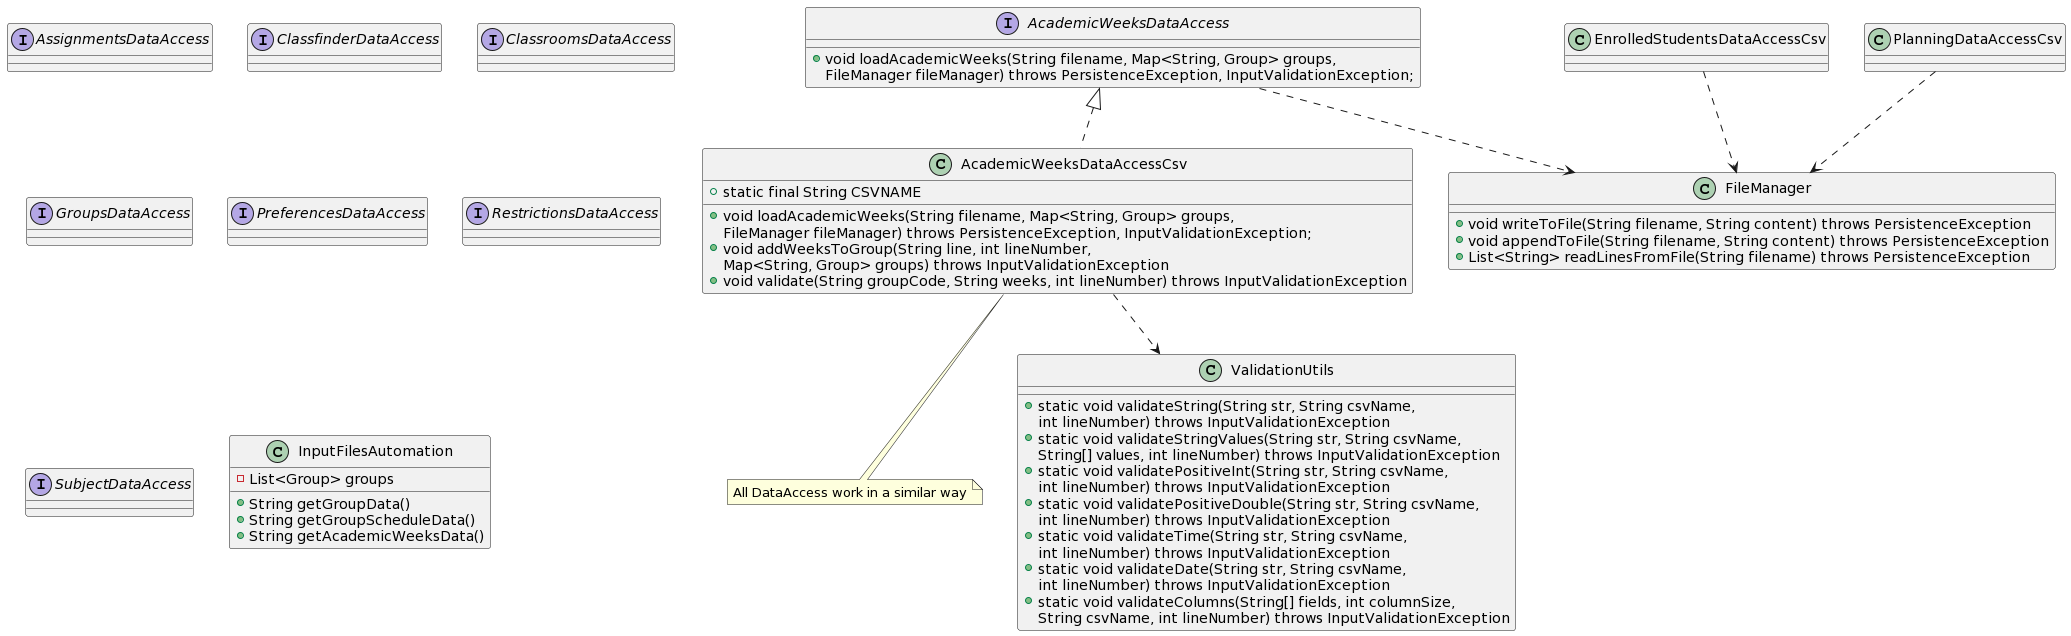
\includegraphics[scale=0.24]{final_persistence_class_diagram_uml.png}
\end{figure}



\section{Interface design}


\section{File format design}

